% !TeX root = ..\..\main.tex
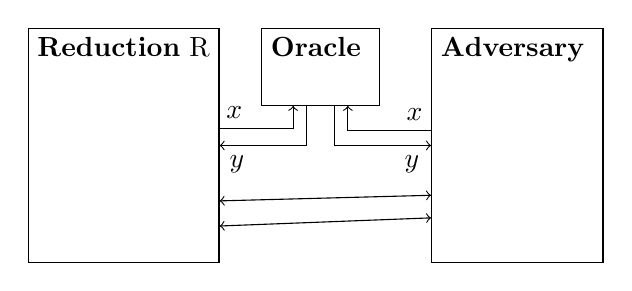
\begin{tikzpicture}
    %draw boxes for reduction oracle and adversary
    %align=left sets the alignment of the text
    %text depth virtually sets the height of the text and therefore shifts the text to the top
    \node[rectangle, draw, minimum width=2cm, align=left, text depth=2.5cm] (R) at (0,0) {\textbf{Reduction} R};
    \node[rectangle, draw, minimum width=1.5cm, align=left, text depth=.5cm] (H) at (2.5,1) {\textbf{Oracle} $\ROh$};
    \node[rectangle, draw, minimum width=2cm, align=left, text depth=2.5cm] (A) at (5,0) {\textbf{Adversary} $\advA$};

    %draw arrows between R and H
    %(R.10) is a border anchor (in angles, i.e. R.0 is at the top center, R.180 at the bottom center)
    %place node above the arrow. pos sets the position from beginning (pos=0) to end (pos=1)
    %using -| instead of -- makes the arrow bend
    \draw[->] (R.10) -| (H.235) node[pos=.1, above] {$x$};
    \draw[<-] (R.0) -| (H.250) node[pos=.1, below] {$y$};

    %draw arrows between H and A
    \draw[->] (A.170) -| (H.305) node[pos=.1, above] {$x$};
    \draw[<-] (A.180) -| (H.290) node[pos=.1, below] {$y$};

    %draw arrows between R and A
    \draw[<->] (R.330) -- (A.210);
    \draw[<->] (R.320) -- (A.220);
\end{tikzpicture}